\documentclass {article}
\usepackage{enumitem}
\usepackage{listings}
\usepackage{color}
\usepackage{float}
\usepackage{mathtools}
\usepackage{graphicx}
\usepackage[hidelinks]{hyperref}
\graphicspath{ {images/} }

\definecolor{mGray}{rgb}{0.39, 0.39, 0.39}
\definecolor{mBlue}{rgb}{0.04, 0.36, 0.67}
\renewcommand*\rmdefault{cmr}

\lstset{ %set options for lstlisting = codesnippets
	basicstyle=\small\ttfamily,
	commentstyle= \small\ttfamily\color{mGray},
	keywordstyle= \color{mBlue},
	numberstyle= \footnotesize\ttfamily\color{mGray},
	breaklines=true,
	captionpos=b,
	numbers=left,
	tabsize=2,
	keepspaces=true,
	showspaces=false,
	showstringspaces=false,
	frame=single
}

\hypersetup{
    colorlinks=false,
}

\setlength{\parindent}{0em}
\setlength{\parskip}{1em}
 
\begin{document}
\begin{titlepage}
	\centering
	
\includegraphics[width=0.3\textwidth]{bth-logo} \par
	{\LARGE A comparison of functional and object-oriented programming paradigms in JavaScript \par}
	\vspace{1cm}
{\large Kim Svensson Sand and Tord Eliasson \par}
{\large \today \par}
	\vfill

	{\normalsize Faculty of Computing \par}
	{\normalsize Blekinge Institute of Technology \par}
	{\normalsize SE-371 79 Karlskrona Sweden \par}
\end{titlepage}
\pagenumbering{gobble}
\newpage
\section*{Abstract}
There are multiple programming paradigms that have their own set rules for how code should be written. Programming languages utilize one or multiple of these paradigms. In this thesis, we will compare object-oriented programming, that is the most used today with languages such as C++ and Java, and functional programming. Functional programming was introduced in the 1950's but suffered from performance issues, and has not been used much except for in the academic world. However, for its ability to handle concurrency and big data, functional programming is of interest in the industry again with languages such as Scala. In functional programming side effects, any interaction outside of the function, are avoided as well as changing and saving state. 

To compare these paradigms we have chosen four different algorithms, which both of us have implemented twice, once according to object-oriented programming and once according to functional programming. All algorithms were implemented JavaScript. JavaScript is a multiparadigm language that supports both functional and object-oriented programming. For all implementations, we have measured development time, lines of code, execution time and memory usage. Our results show that object-oriented programming gave us better performance, but functional programming resulted in less code and a shorter development time. 
\subsection*{Keywords}
Functional programming, Object-oriented programming, Comparison, Programming paradigms, JavaScript

\newpage
\tableofcontents
\newpage
\pagenumbering{arabic}
\newpage
\listoffigures
\newpage
\listoftables
\newpage
\section*{Abbreviations}
\begin{itemize}[leftmargin=*]
\item [ ] ES6 = ECMAScript 2015
\item [ ] FP = Functional Programming
\item [ ] OOP = Object-Oriented Programming
\item [ ] RP = Reactive Programming
\end{itemize}

\newpage
\section{Introduction}
Programming paradigms is a way to classify a certain way of programming \cite{programming-paradigms}. Each paradigm has its own set of rules for how the code should be written. Some programming languages make it possible to write code according to one paradigm,  while others make it possible to write according to multiple paradigms. 

In the 1950's and 60's, multiple high-level languages were developed that today's programming languages are based upon \cite{gabmar}. These were imperative languages such as Fortran and Algol, functional languages such as Lisp and object-oriented languages such as Simula. Originally Lisp had performance issues and has not been used a lot commercially, but versions of it are still used today. However, it is mostly used an academic context. In the 70's, C was introduced and quickly established itself thanks to its ability to access low-level functionality, its compact syntax and its effective compiler. In the 80's, the object-oriented language C++ was developed. It was based on C and and took a lot of inspiration from Simula. Java, that is based on C++ was introduced in the 90's. Since imperative languages gained the upper hand in the 60's and 70's, new languages were based on those and continued being the most used. 

Object-oriented or imperative languages are dominating today, with languages such as C, C++, Java and C\#. However, functional languages seem to be of interest in the industry again for handling big data and concurrency, with languages such as Scala, Erlang and Haskell \cite{drboolean, eriksen, erikarl}. Since functional programming tries to avoid state, it becomes less complex to run asynchronous and therefore easier to run concurrently. There is a performance difference, where functional languages tend to be slower, but there are also positive aspects that could compensate for those, such as memory usage and less code \cite{fogus, alomgi}.  Some are also arguing that a more functional approach will give you more readable code, code that is easier to maintain and easier to test, and that learning it will give you a better experience as a programmer \cite{drboolean, meijer}. 

We will compare two programming paradigms, object-oriented programming and functional programming. To compare these, we have chosen four different algorithms which both of us will implement twice, once according to the object-oriented paradigm and once according to the functional paradigm. The different algorithms we will implement are binary search tree algorithms, the Shellsort algorithm, the Tower of Hanoi algorithm and Dijkstra's algorithm. The comparisons we will make between the algorithms are execution time, memory usage, development time and lines of code. All algorithms will be written in JavaScript.
\subsection{Research Questions}
In this thesis we will address the following research questions:
\begin{itemize}
\item Will functional versus object-oriented approaches in JavaScript have an impact on performance, such as execution time and memory usage?
\item Can programmers with an object-oriented background decrease development time by using practises from functional programming?
\end{itemize}

When comparing the different paradigms, it would be interesting to see how the execution time and memory usage differs. Because we are writing both paradigms in the same language, we are able to compare just the paradigms, without having to compare languages and compilers.

We both have studied at Blekinge Institute of Technology, where we learned object-oriented programming, OOP. Therefore, it would be interesting to see how our programming will change by learning functional programming, FP. This can give teachers an indication about introducing functional programming, to give students a chance to use different paradigms depending on their needs, instead of always using OOP.
\section{Background and Related work}
Here we will describe the functional programming paradigm and also the object -oriented programming paradigm. We will also describe JavaScript and its support for functional and object-oriented methods. The related works described are articles that further explain the positive aspects of functional programming or studies similar to this one.
\subsection{Functional programming}
Functional programming is a programming paradigm that at its core is based on lambda-calculus \cite{gabmar}. Programs are constructed using functions and by avoiding changing the state. By not modifying the state side effects are avoided. Computation is done by changing the environment, rewriting the functions, rather than changing variables. Multiple functions can be composed into larger and more complex functions, and should be reduced to its simplest state following mathematical rules. The following are concepts used in FP:
\begin{description}
\item [Lazy evaluation] - Lazy evaluation is when a value is not calculated until it is needed \cite{fogus}.
\item [Static type checking] - Pure functional languages usually have static type checking \cite{gabmar}. This means that variables are of a certain type, for example int or char. In such languages it is not allowed to use functions or variables with the wrong types. So if there is, for example, a function taking an int as parameter it is illegal to call that function with a String as its parameter. In dynamically type checked-languages this would be legal at compile time, since variables are not specified as types, but would cause an unexpected error at runtime. For example in JavaScript:

\begin{lstlisting}[language=Java]
//JavaScript has dynamic type checking
function double(nr) {
  return nr * 2;
}

var word = "string";
double(word); //Will return NaN but still continue running
\end{lstlisting}

\item [ ] A similar program in golang \cite{golang}, that is a statically type checked language:

\begin{lstlisting}[language=Java]
func main() {
  var word string = "string"
  fmt.Printf("%d", double(word)) //Error: cannot use word (type string) as type int in argument to double
}

func double(nr int) int {
  return nr * 2
}
\end{lstlisting}

\item [ ] This will give an error when compiling.
\item[] There are however pure functional languages with dynamic type checking, such as Clean \cite{clean}. There are also languages that are mostly functional with dynamic type checking, such as Common Lisp \cite{commonLisp} or Scheme \cite{scheme} \cite{langTable}.
\item [Side effects] - Side effects are for example changing a variable or having some interaction outside of the function \cite{drboolean}. This is avoided in functional programming since it may result in incorrect and unexpected behaviour. 
\item [Pure functions] - A pure functions always returns the same result, given the same input, and does not have side effects \cite{drboolean}. See the following example: 

\begin{lstlisting}[language=Java]
var sum = 0;

//Impure
function add(a, b) {
  sum = a + b;
}

//Pure
function add(a, b) {
  var tmp = a + b;
  return tmp;
}
\end{lstlisting}

\item [Higher order functions] - Higher order functions are an important concept in functional programming \cite{fogus}. First class functions mean that functions are treated as values, which means that they can be stored in variables and arrays or created if needed. A higher order function is a first class function that either takes a function as a parameter, returns a function as a result or both. This makes it possible to compose larger and more complex functions.

\begin{lstlisting}[language=Java, breaklines=true]
function add(a, b) {
  return a + b;
}

//Functions can be placed in variables.
var thisFunc = add;

//And also put in other variables.
var sameFunc = thisFunc;
sameFunc(1, 2); //Will give the output 3.

//Functions can also be used as parameters or return values.
function applyFunc(f, a, b) {
  return f(a, b);
}

applyFunc(function(a, b) {
  return a * b;
}, 3, 2); //Will give output of 6

//Returns a function that returns a string
function getStringCreator(category, unit) {
  return function(value) {
    return category + ': ' + value + unit;
  }
}

var weightStringCreator = getStringCreator('Weight', 'kg');
weightStringCreator(5); //Outputs "Weight: 5kg"
\end{lstlisting}

\item [Recursion] - Recursive functions are functions that call themselves and are used as loops \cite{fogus}. It is important in functional programming since it can hide mutable state and also implement laziness. In functional programming loops are avoided and recursion is used instead.

\begin{lstlisting}[language=Java]
//Adds all numbers from start to end with a loop
function iterativeAdd(start, end) {
  var sum = 0;
  while(start <= end) {
    sum += start;
    start++;
  }

  return sum;
}

//Adds all numbers from start to end recursively
function recursiveAdd(start, end) {
  if (start == end) {
    return end;
  }
  else {
    return start + recursiveAdd(start + 1, end);
  }
}
iterativeAdd(1, 6); //Outputs 21
recursiveAdd(1, 6); //Also outputs 21
\end{lstlisting}

\item [Currying] - Currying means a function can be called with fewer arguments than it expects and it will return a function that takes the remaining arguments \cite{drboolean}. 

\begin{lstlisting}[language=Java, breaklines=true]
//Returns a new function that takes the remaining argument or the sum of a and b if both are provided.
function addWithCurrying(a, b) {
  if(b) {
    return a + b;
  }
  else {
    return function(b) {
      return a + b;
    }
  }
}

var curryAdd = addWithCurrying(4); 
curryAdd(6); //Outputs 10
addWithCurrying(4, 6); //Also outputs 10
\end{lstlisting}

\item [Immutable data structures] - In functional programming mutations, that are side effects, are avoided \cite{fogus}. Hidden side effects can result in a chains of unpredicted behaviour in large systems. Instead of mutating the data itself a local copy is mutated and returned as a result, as seen in the pure functions example. In languages with immutable data structures it is illegal to change the value of such variables.
\end{description}
\subsection{Object-oriented programming}
Object-oriented programming is a programming paradigm which is built around "objects". These objects may contain data, in the form of fields often referred to as attributes, and code, in the form of procedures often referred to as methods \cite{kindler}.

These objects are created by the programmer to represent something with the help of its attributes and methods. What kind of variables and functions an object should contain is defined in a class, which works like a blueprint for the object. For example, a class can represent an employee, see figure~\ref{fig:oop-example}. An employee has the attributes name, assignment and salary. The employee also has a method for doing work. Then the employee has to work somewhere, so we create another object for a company where our employee can work. The company has the attributes name, income and number of employees. It also has methods to hire employees and fire employees. Since there are more employees who works at this company, we can add more employees by creating new objects of the employee class.

\begin{figure}[H]
\centering
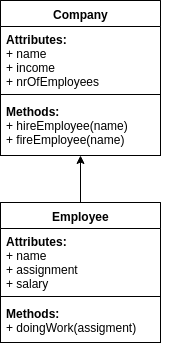
\includegraphics[width=0.3\textwidth]{oop-example}

\caption {OOP example}
\label{fig:oop-example}
\end {figure}

By creating classes and object like this, you can create programs according to the object-oriented paradigm.

The following are concepts used in OOP:
\begin{description}
\item [Class] - A class is a model for a set of objects, which the object oriented paradigm is built around \cite{gabmar}. The class establishes what the object will contain, for example variables and functions, and signatures and visibility of these. To create an object of any kind a class must be present. 

\begin{lstlisting}[language=Java]
//Creates a class Animal with the properties name and age and a function for logging the properties to the screen
class Animal {
  constructor (name, age) {
    this.name = name;
    this.age = age;
  }

  logAnimal() {
    console.log('Name: ' + this.name + '\nAge: ' + this.age);
  }
}

var animal = new Animal('Buster', '9');
animal.logAnimal();
//Outputs Name: Buster
//Age: 9
\end{lstlisting}
\item [Object] - An object is a capsule that contains the structure of variables and functions established in the class\cite{gabmar, skansholm}. While the structure looks the same in objects created with the same class, the containing information can vary.
\item [Inheritance] - When an object acquires all properties and functionality of another object it is called inheritance \cite{skansholm}. This provides code reusability. 

\begin{lstlisting}[language=Java, breaklines=true]
//Based upon the Animal class with an added property race
//The original logAnimal() is overidden so the new property is also logged to the screen.
class Dog extends Animal {
  constructor(name, age, race) {
    super(name, age);
    this.race = race;
  }

  logAnimal() {
    super.logAnimal();
    console.log('Race: ' + this.race);
  }
}

var dog = new Dog('Buster', '9', 'Shitzu');
dog.logAnimal();
//Outputs Name: Buster
//Age: 9
//Race: Shitzu
\end{lstlisting}

\item [Encapsulation] - Encapsulation can be used to refer to two different things. A mechanism to restrict direct access to some object components and the language construct that facilitates the bundling of data with methods \cite{gabmar, skansholm}. Access to variables and functions are established in the class by using the private and public keyword. The bundling is the object itself.

\item [Polymorphism] - When a method is used in different ways it is called polymorphism \cite{gabmar, skansholm}. This is achieved with the help of overloading and overriding.

\item[Overloading] - Refers to creating a function with the same name as another function, often very similar, with either different types of variables in the parameters or different number of parameters \cite{skansholm}.

\item[Overriding] - Refers to overwriting a function written in a superclass to make it do something else than first intended, without changing the superclass \cite{skansholm}.
\end{description}
\subsection{JavaScript}
\label{sec:javascript}
JavaScript is a language with first class functions that is dynamically type checked. It is a multi-paradigm language with basic support for object-oriented, imperative and functional paradigm principles. There are multiple libraries to tweak JavaScript with certain functions or better support for certain paradigms, for example Underscore.js \cite{underscorejs}, for functional programming, or Flow \cite{flow}, for static type checking. There are also a lot of languages available that are transpiled into JavaScript, for example TypeScript \cite{typescript}. 

JavaScript can be run in most browsers and also in servers and is implemented to follow the ECMA standards \cite{ecma6table}. It has a garbage collection system for handling memory \cite{mozillamem}. The garbage collection removes objects or variables from memory that are unreachable by the program. 

Objects in JavaScript are treated as references. When an object is initiated to a variable it is created and placed in memory and the variable is given a reference to it. This means that if another variable is assigned this object, it gets a copy of the reference to it, rather than a copy of the object itself. Arrays are objects in JavaScript and will be treated the same way.

\begin{lstlisting}[language=Java, breaklines=true]
//JavaScript Object handling
var array = [1, 2, 3, 4, 5, 6, 7, 8, 9, 10];
var obj = {
  text: 'Some text'
}

var arrayRef = array;
var objRef = obj;

// Gets references to original array and object.
console.log(arrayRef); // [ 1, 2, 3, 4, 5, 6, 7, 8, 9, 10 ]
console.log(objRef); // { text: 'Some text' }

// Change stuff
arrayRef.pop();
objRef.text = 'Some other text';

// Mutating new variables mutates original objects.
console.log(array); // [ 1, 2, 3, 4, 5, 6, 7, 8, 9 ]
console.log(obj); // { text: 'Some other text' }
\end{lstlisting}
\subsubsection{Functional programming}
\label{sec:js-fp}
JavaScript is not a functional language, but it is possible to write functional code with it \cite{drboolean}. There are also libraries that makes functional programming in JavaScript easier, such as Underscore.js \cite{underscorejs} \cite{fogus}. However, we will use ECMA 2015, ES6, that already provide many of the functions provided by Underscore.js. This is also to use the same environment for our different implementations in this experiment.

In JavaScript it is possible to treat functions as any other variable, pass them as function parameters or store them in arrays, so called first class functions \cite{drboolean}. There are also higher order functions such as map(), filter() and reduce() that might replace loops \cite{grady}:

\begin{description}
\item [map()] - Calls a provided function on every element in an array and returns an array with the outputs \cite{jsref}.
\item [filter()] - Returns a new array with all the elements that passes a test in a provided function. 
\item [reduce()] - Reduces an array to a single value.
\end{description}

However there is no automatic currying or immutable data structures in JavaScript. JavaScript is also dynamically type checked. These can be added to JavaScript with libraries.

There is a call stack limit in JavaScript that varies depending on the runtime environment. This limits the number of function calls that can be made, which also limits recursion. In ES6 there is tail call optimization, that makes it possible to make certain function calls without adding to the call stack, that would allow for better recursion. However this is currently not implemented for most servers and browsers \cite{ecma6table}.
\subsubsection{Object-oriented programming}
JavaScript has always had support for OOP. But 
with ES6, OOP in JavaScript starts to look more like classical OOP languages such as Java \cite{ecmacompare}.

JavaScript do not fully support encapsulation, since you can't make variables and functions private or public. Otherwise there is full support for OOP in JavaScript. As a workaround many programmers add an underscore to the variable or function name. This, however, does not actually make anything private. It just gives a hint to the programmer that it should be treated as such.
\subsection{Related work}
In "Curse of the excluded middle" \cite{meijer} Erik Meijer argues, with multiple examples, that the industry should not focus on a combination between functional and objected oriented methods to counter handling big data with concurrency. He concludes that it is not good enough to avoid side effects in imperative or object-oriented languages. It is also not good enough to try to ignore side effects in pure functional languages. Instead he thinks that people should either accept side effects or think more seriously about using the functional paradigm.

In "Functional at scale" \cite{eriksen} by Marius Eriksen he is explaining why Twitter uses methods from functional programming to handle concurrent events that arises in large distributed systems in cloud environments. In the functional programming paradigm it is possible build complex parts out of simple building blocks, thus making systems more modular. He concludes that the functional paradigm has multiple tools for handling the complexity present in modern software.

Eriksson and \"{A}rleryd are looking at how to use functional practises, such as immutable data structures, pure functions and currying, when developing front end applications by taking inspiration from Elm \cite{elm} in their master's thesis \cite{erikarl}. They have researched each practise in Elm to see if it is possible to use these practises in JavaScript together with tools and libraries. Their conclusion was that it is possible to replicate functional practises from Elm in JavaScript, but that they prefer working with Elm. In JavaScript multiple libraries had to be included to use the same practises. They also concluded that even though functional programming is not widely used within the industry, functional practises can still be used in all projects.

In "Improving Testability and Reuse by Transitioning to Functional Programming" \cite{benrad}, Benton and Radziwill state that functional programming is better suited for test driven development (TDD) and concludes that a shift toward the functional paradigm benefits reuse and testability of cloud-based applications.

Alic, Omanovic and Giedrimas have made a comparative analysis of functional and object-oriented programming languages \cite{alomgi}. They have compared four languages, C\#, F\#, Java and Haskell based on execution time and memory usage. Their conclusion is that Java is the fastest while Haskell uses much less memory, and that programming paradigms should be combined to increase execution efficiency. 

Dobre and Xhafa writes in "Parallel Programming Paradigms and Frameworks in Big Data Era" that we now are in a big data era \cite{dobre}. They also review different frameworks and programming paradigms in a big data perspective. Regarding paradigms they state: "functional programming (FP)  is actually considered today to be the most prominent programming paradigm, as it allows actually more flexibility in defining big data distributed processing workflows" \cite{dobre}.

In "Comparing programming paradigms: an evaluation of functional and object-oriented programs", R. Harrison et al. compares the quality of code in functional and object-oriented programming \cite{hasmadole}. To compare these, they use C++ and SML. While they state in their discussion that they would probably use OOP, since C++ is a better language, the standard list functions were of great help, the debugging was better and reusability was much higher in SML.

Guido Salvaneschi et al. have conducted an empirical evaluation of the impact of Reactive Programming (RP), with functional programming concepts, on program comprehension \cite{saproamname}. Their experiment involved 127 subjects and the results suggest that RP is better for program comprehension when compared with OOP. They conclude that with RP the subjects produced more correct code without the need of more time, and also that the comprehension of RP programs is less tied to programming skills. 

In "Using Functional Programming within an Industrial Product Group: Perspectives and Perceptions" \cite{scomad}, David Scott et al. presents a case-study of using FP in the multiparadigm language OCaml in a large product development team. They found that the team's project was a success even though there were some drawbacks to using OCaml, such as lack of tool support. The engineers believed that OCaml enabled them to be more productive than if they would have used one of the mainstream languages, such as C++ or Python.
\section{Method}
In this experiment each person will implement four different algorithms, once with FP and once with OOP. We have chosen algorithms that are well known, so that our focus will be on the different implementations, rather than on how the algorithms work. For each of these algorithms we will measure execution time, memory usage, development time and lines of code. The way the algorithms should be implemented and paradigm guidelines are also defined.
\subsection{Algorithms}
We will implement binary search tree algorithms, the Shellsort algorithm, the Tower of Hanoi algorithm and Dijkstra's algorithm. One of the binary search tree algorithms we will implement is in-order tree traversal, which is a recursive algorithm, as is the Tower of Hanoi algorithm. These algorithms fit well for FP since they use recursion. The implementation of the binary tree structure can however be implemented by using classes and objects, that are used in OOP. Shellsort uses state and iteration which is used in OOP and avoided in FP. Dijkstra's algorithm also uses state and iteration, and the graph can also be implemented using classes and objects.

We chose algorithms that use both recursion and iteration to not give advantage to any paradigm. When implementing these algorithms and data structures we can also make use of OOP methods, such as classes and objects. The algorithms' purpose are also different to avoid for example implementing four different sorting algorithms. 
\subsubsection{Binary search tree algorithms}
\label{sec:binary-tree}
A binary tree is a tree consisting of nodes, where a node can have a maximum of two children \cite{weiss}. These children can be described as the left and the right subtree. The property that differs a binary search tree from a standard binary tree, is the order of the nodes. In a binary tree the order can be undecided, but in a binary search tree the nodes are stored in an order based on some property. For example in our binary search tree the left subtree of a root will contain smaller numbers than the root, and the right subtree will contain larger numbers. See the example in figure~\ref{fig:binary-tree-example}. Using tree traversal it is possible to find certain nodes or get a list of sorted objects. Our binary search tree will contain random numbers and the functions:
\begin{description}
\item [findNode(comparable, rootNode)] - Finds a specific key in the tree.
\item [inOrderTraversal(root)] - Returns an array of all numbers in the tree, sorted smallest to biggest.
\item [insert(comparable, rootNode)] - Inserts number into the tree. Returns true or false depending on success. If comparable is already in the tree, false should be returned. Note that in the functional implementation this function will return the resulting tree instead of mutating the tree and returning true or false.
\end{description}

\begin{figure}[H]
\includegraphics[width=\textwidth]{binary-tree-example}


\caption {Binary tree example}
\label{fig:binary-tree-example}
\end {figure}

\begin{description}
\item[Algorithm descriptions:]
\item [algorithm findNode(comparable, root)]
\item[]
\begin{lstlisting}[language=Pascal]
if root is undefined then
  return null
else if comparable is equal to comparable in root then
  return root
else if comparable is larger than comparable in root then
  return findNode(comparable, rightSubtree in root)
else if comparable is smaller than comparable in root then
  return findNode(comparable, leftSubtree in root)
end if
\end{lstlisting}

\item [algorithm inOrderTraversal(root)]
\item []
\begin{lstlisting}[language=Pascal]
set array to empty array
if comparable in root is undefined then
  return array
else then
  add inOrderTraversal(leftSubtree in root) to end of array
  add comparable in root at end of array
  add inOrderTraversal(rightSubtree in root) at end of array
  return array
end if
\end{lstlisting}

\item[] Running this on the tree in figure~\ref{fig:binary-tree-example} would return the array [8, 10, 15, 18, 24, 22, 31, 39, 48, 52, 56, 71, 84, 88, 90, 93].

\item [algorithm insert(comparable, root)]
\item []
\begin{lstlisting}[language=Pascal]
if comparable is equal to comparable in root then
  return false
else if comparable is larger than comparable in root then
  if rightSubtree in root is undefined then
    create newNode
	  set comparable in newNode to comparable
    set rightSubtree of root to newNode
    return true
  else then
    return insert(comparable, rightSubtree in root)
  end if
else if comparable is smaller than comparable in root then
  if leftSubtree in root is undefined then 
    create newNode
    set comparable in newNode to comparable
    set leftSubtree in root to newNode
    return true
  else then
    return insert(comparable, leftSubtree in root)
  end if
end if
\end{lstlisting}
\end{description}
\subsubsection{Shellsort algorithm}
The Shellsort algorithm is named after its creator Donald Shell \cite{weiss}. It was one of the first algorithms to break the quadratic time barrier. The algorithm sorts by sorting items using insertion sort with a gap. For each run the gap is decreased until the gap is 1 and the items are sorted. How the gap is decreased is decided with a gap sequence. Different gap sequences gives Shellsort a different worst-case running time.
 
We will use one of Sedgewick's gap sequences that give Shellsort one of the fastest worst-case running times, \(O(n^3/4)\).

The sequence is 

\(\{1, 5, 19, 41, 109...\}\), where every other term is of the form

\(9 * 4^k - 9 * 2^k + 1\), and every other term is of the form

\(4^n - 3 * 2^n + 1\), where 

\(k = {0, 1, 2, 3...}\) and \(n = {2, 3, 4, 5...}\).
 
In our implementations the sequence is calculated during execution and included in our measurements.

This algorithm will sort an array filled with randomized numbers. Our implementation uses this algorithm in a function:

\begin{description}
\item[Shellsort(array)] - Takes an unsorted array as an input and returns a sorted copy of the array. 

\item[Algorithm description:]
\item[algorithm algorithm Shellsort(array of size n)]
\item []
\begin{lstlisting}[language=Pascal]
set sortedArray to array
set gapSequence to Sedgewicks gap sequence
set currentGapIndex to 0
set currentGap to the largest gap i gapSequence where gap is smaller than n divided by 2
set currentGapIndex to the index of currentGap in gapSequence

while currentGap is larger than 0 do
  for i = currentGap to n
    set currentValue to array[i]
    set currentIndex to i
    while currentIndex - currentGap is larger or equal to 0 and sortedArray[currentIndex - currentGap] is larger than currentValue do
      set sortedArray[currentIndex] to sortedArray[currentIndex - currentGap]
      set currentIndex to currentIndex - currentGap
    end while
    set sortedArray[currentIndex] to currentValue
  end for
  set currentGapIndex to currentGapIndex - 1
  set currentGap to gapSequence[currentGapIndex]
end while
return sortedArray
\end{lstlisting}
\end{description}
\subsubsection{The Tower of Hanoi algorithm}
\label{sec:hanoi}
The Tower of Hanoi is a game invented by mathematician \`{E}douard Lucas in 1883 \cite{hanoi}. The game consists of three pegs and a number of disks stacked in decreasing order on one of the pegs, see figure~\ref{fig:tower-of-hanoi-example}. The goal is to move the tower from one peg to another by moving one disk at a the time to one of the other pegs. A disk can not be placed on a peg on top a smaller disk. 

\begin{figure}[H]
\includegraphics[width=\textwidth]{tower-of-hanoi-example}

\caption{Tower of Hanoi image}
\label{fig:tower-of-hanoi-example}
\end{figure}

This algorithm will move a tower from one peg to another in the function:

\begin{description}
\item[hanoi(tower, start, dest, aux)] - Moves tower from start to dest following the rules of the Tower of Hanoi problem. Returns the start, dest and aux pegs with the repositioned tower.


\item[Algorithm description:]
\item[algorithm hanoi(tower, start, dest, aux)]
\item[] 
\begin{lstlisting}[language=Pascal]
(*Pseudo code based on that tower is the number of the largest disk, where 1 is the smallest disk in the tower.*)
if tower is equal to 1
  move tower from start to dest
else
  hanoi(tower - 1, start, aux, dest)
  move tower from start to dest
  hanoi(tower - 1, aux, dest, start)
end if
\end{lstlisting}
\end{description}
\subsubsection{Dijkstra's algorithm}
Dijkstra's algorithm is an algorithm for finding the shortest path in a graph consisting of a number of nodes connected by edges \cite{weiss}, where the weight of the edges is known, see figure~\ref{fig:dijkstras-algorithm-example1}. The algorithm will find the shortest path from the start node to the end node in a graph. It is initiated by:
\begin{enumerate}
\item setting the distance to the start node to 0.
\item setting the distance to all other nodes to infinity.
\item mark all nodes as unvisited.
\end{enumerate}
The algorithm will then find the shortest path using the following steps:
\begin{enumerate}
\item Set current node to the node with the smallest distance that has not already been visited.
\item For all neighbors to current node that has not already been visited, check if their distance is smaller than the distance of current node + the distance to the neighbor. If so, update the distance of the neighbor.
\item Mark current node as visited.
\item Repeat until all nodes have been visited or the end node has been visited.
\end{enumerate}
See the result in figure~\ref{fig:dijkstras-algorithm-example2}.

\begin{figure}[H]
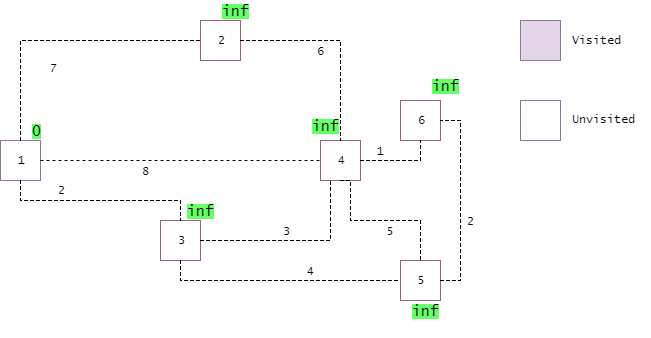
\includegraphics[width=\textwidth]{dijkstras-algorithm-example1}


\caption{After initiation of Dijkstra's algorithm}
\label{fig:dijkstras-algorithm-example1}
\end{figure}
\begin{figure}[H]
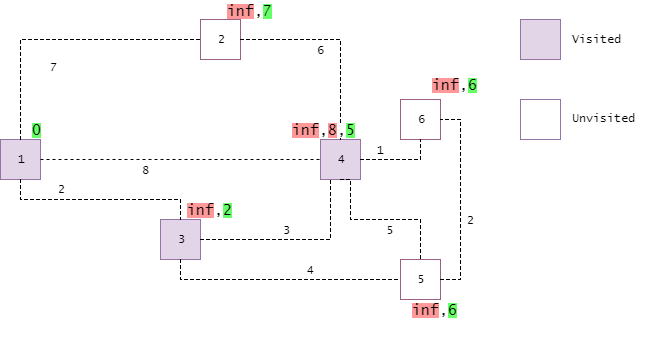
\includegraphics[width=\textwidth]{dijkstras-algorithm-example2}

\caption{After three nodes have been visited with Dijkstra's algorithm}
\label{fig:dijkstras-algorithm-example2}
\end{figure}

This algorithm will be used in a function:
\begin{description}
\item[dijkstras(graph, startNode, endNode)] - That takes graph, startNode and endNode and returns an array with the shortest path from startNode to destNode. 

\item [Algorithm description:]
\item[algorithm dijkstras(graph, startNode, endNode)]
\item[]
\begin{lstlisting}[language=Pascal]
for each node in graph
  set dist[node] to infinity
  set path[node] to undefined
end for
set dist[startNode] to 0
set unvisitedNodes to nodes in graph

while unvisitedNodes is not empty or endNode is not in unvisitedNodes do
  set current to node where dist[node] is smallest and node is in unvisitedNodes 
  remove current from unvisitedNodes
  for each neighbor of current where neighbor is in unvisited do
    set temp to dist[current] + weight of edge in graph, where edge is from current to neighbor
    if temp is smaller than dist[neighbor] then
      set dist[neighbor] to temp
      set path[neighbor] to path[current] + current
    end if
  end for
end while
return path[endNode]
\end{lstlisting}
\end{description}
\subsection{Environment}
We will implement the algorithms using Atom \cite{atom}, a text editor, and compile and run our tests and our code with Node.js \cite{nodejs}. Tail call optimization is not available in Node.js, see \ref{sec:js-fp}. To manage our dependencies we are using npm \cite{npm} and for automation we are using Grunt \cite{grunt}. We have been using github for managing and reviewing our code, see \url{https://github.com/KimSvenSand/ToKi}.

Since Node.js does not support ES6-modules we are using Babel \cite{babel} to transpile our ES6-modules to node-modules that are supported. We are doing this since we have prior experience with ES6 modules and not with node-modules. Since Node.js supports almost everything else in ES6 we will only be transpiling the modules, leaving our code in an ES6 standard.

To measure memory and run time we are using Node.js' process, that is a global variable and therefore always available within Node.js applications \cite{nodejs}. We are using the following functions:
\begin{description}
\item [process.hrtime(time)] - Returns the current high resolution time in a [seconds, nanoseconds] tuple Array. If the optional time-parameter, an earlier hrtime, is used, it will return the difference between that time and the current time. These times are relative to an arbitrary time in the past, and not related to the time of day and therefore not subject to clock drift.
\item [process.memoryUsage()] - Returns an object describing the memory usage of the Node.js process measured in bytes.
\end{description}
\subsection{Testing}
Our code will be tested through code reviews and unit testing.
\subsubsection{Code reviews}
We will review each other's implementations and our implementations will also be reviewed by a third party. The reviews should help us to find bugs and also to confirm that we have used FP or OOP methods according to our guidelines, see \ref{sec:paradigm-guidelines}.
\subsubsection{Unit testing}
Unit testing will be done using the JavaScript libraries Mocha \cite{mocha} for writing tests and Chai \cite{chai} for evaluating expressions. Our implementations will have to pass the tests in appendix~\ref{appendix:test-cases} to be accepted as done.
\subsection{Implementation}
We will proceed from a template with the following structure:

\begin{lstlisting}[language=Pascal, deletekeywords={function, and}, numbers=none]
|---dist
|   \---<Files generated from babel>
|---src
|   |---js
|        |---<function and class files>
|   \---index.js
|---es6-test
|   \---<Test files>
|---test
|   \---<Test files generated from babel>
| Gruntfile.js
| package.json
\end{lstlisting}

\begin{description}
\item[] To run our tests we use the command:
\item[npm test] - Will transpile the test files in the es6-test-folder, place the generated files in the test-folder and run the tests.
\item[] To execute our code we use the command:
\item[npm start] - Will transpile the JavaScript-files in src-folder, place the generated files in the dist-folder and run index.js in the dist-folder.
\end{description}

For an implementation of an algorithm to be considered done the following has to be implemented and provided:
\begin{itemize}
\item Tests for the algorithm that are defined in appendix~\ref{appendix:test-cases} placed in \(<\)projectName\(>\)/es6-test
\item A complete implementation of the algorithm that has passed the tests placed in \(<\)projectName\(>\)/src/js
\item A measurement implementation that must run the algorithm and measure time and memory usage using Node.js process. The implementation must have a function for creating randomized data of a certain size according to table~\ref{tab:measurements} 
\item A timelog describing how long the implementation took. 
\end{itemize}
\subsection{Measurements and indata}
We will measure execution time, memory usage, code length and the development time of each implementation. The measurements are done on the algorithms described earlier in this chapter and the algorithms will run on randomized data, described in table~\ref{tab:measurements}. We are not measuring the initiation of the randomized data, except for the binary search tree algorithms that include an insert-function. The algorithms are measured with three different sizes of data, described in table~\ref{tab:measurements}, to get more accurate results. We have chosen measurement sizes such as to avoid exceeding the call stack limit for our functional implementations, that use recursion.

\begin{table}[H]
\caption{Table describing measurements to be implemented}
\begin{tabular}{ | l p{10cm} | }
\hline
Algorithm & Binary search tree algorithms \\
Description & Should measure insert(), inOrderTraversal() and findNode(), where findNode() is run three times with a random value between 1 and 10 * n as parameter. \\
Measurement data & A binary search tree with n nodes filled with randomised values between 1 and 10 * n. \\ 
Measurement sizes & n = 1000, n = 5000 and n = 10000. \\
\hline
Algorithm & Shellsort algorithm \\
Description & Should measure the Shellsort-function.\\
Measurement data & An array of length n filled with randomised values between 1 and 2 * n \\ 
Measurement sizes & n = 1000, n = 3000 and n = 6000. \\
\hline
Algorithm & Tower of Hanoi algorithm \\
Description & Should measure the hanoi-algorithm where a tower is moved from one peg to another. \\
Measurement data & A tower of n disks. \\ 
Measurement sizes & n = 10, n = 20 and n = 25. \\
\hline
Algorithm & Dijkstra's algorithm \\
Description & Should measure Dijkstra's algorithm from the first node in the randomised graph to the last node in the randomised graph.\\
Measurement data & A graph with n nodes where each node is connected to the last two nodes, if those nodes exist. The edges between the nodes should be of a randomised weight between 1 and 100.\\ 
Measurement sizes & n = 10, n = 15 and n = 20. \\
\hline
\end{tabular}
\label{tab:measurements}
\end{table}
\subsection{Guidelines for implementations and reviews}
\label{sec:guidelines}
The following are guidelines for when the algorithms are implemented. They will also work as criteria for the implementations when reviewing, and has to be fulfilled for the implementation to be approved.
\label{sec:paradigm-guidelines}

\textbf{Functional programming guidelines:}
\begin{itemize}
\item Do not use classes
\item Treat functions as variables
\item Compose functions to build programs
\item Use already provided pure functions when possible
\item Write pure functions
\item Do not change variables
\item Use recursion instead of iteration
\end{itemize}

\textbf{Object-Oriented Programming guidelines:}
\begin{itemize}
\item Use classes and objects to build programs
\item Use inheritance when possible
\item Use encapsulation
\item Each class should have only one job
\item Prefer iteration over recursion
\end{itemize}

\section{Results and analysis}
Our implementations have been reviewed by each other and also by Emil Folino who is a lecturer at BTH. During reviews we focused on finding any deviation from the guidelines, see section~\ref{sec:guidelines}, and finding larger bugs and mistakes. Small bugs were intended to be found using our tests, see appendix~\ref{appendix:test-cases}, but a few bugs still slipped through and had to be fixed. They were found when we noticed some strange results that we could not explain. For some of our implementations we had made mistakes when implementing the index-files, that ran the measurements, and these were not included in our tests.

All of our code is available at \url{https://github.com/KimSvenSand/ToKi}
\subsection{Development time}
\label{sec:development-time}
The total results for the development time were:
\begin{description}
\item[Kim OOP] - 21 hours and 12 minutes.
\item[Kim FP] - 19 hours.
\item[Tord OOP] - 24 hours and 22 minutes.
\item[Tord FP] - 22 hours and 36 minutes.
\end{description}

In figure~\ref{fig:development-time-graph} we can see that both of us spent less time on the functional implementations in total. We both had to spend more time on the OOP solution when implementing the recursive algorithms and vice versa. This is true except for Dijkstra's algorithm where Tord spent about as much time on both of the implementations. 

Tord had to redo both of his Dijkstra's algorithm implementation, the functional Shellsort algorithm and the object-oriented Tower of Hanoi after the initial results were registered. He spent a lot of time finding and fixing the bug for his functional Dijkstra's algorithm, which explains the deviation from the expected pattern.

We can see that there was a large difference in development time between Kim's functional and object-oriented Tower of Hanoi algorithm. We can also see that she spent a lot more time than Tord did on his Tower of Hanoi implementations. This was because she struggled a lot with the iterative Tower of Hanoi algorithm and chose to use data structures where the algorithm had to be altered from the pseudocode in section~\ref{sec:hanoi}. Another difference between Kim's and Tord's implementations was that Tord got stuck and searched for help online regarding the iterative Tower of Hanoi algorithm.

We hoped that we would see a clear advantage for FP, but there is only a slight difference when looking at the total hours spent on each paradigm. The results suggest that the major difference in development time is depending on the algorithm itself and how it is implemented, rather than on the paradigm that is used. However, both of us have had prior experience working with OOP and close to no experience working with FP. This could mean that FP has a larger advantage than what is apparent in our results. 

\begin{figure}[H]
\centering
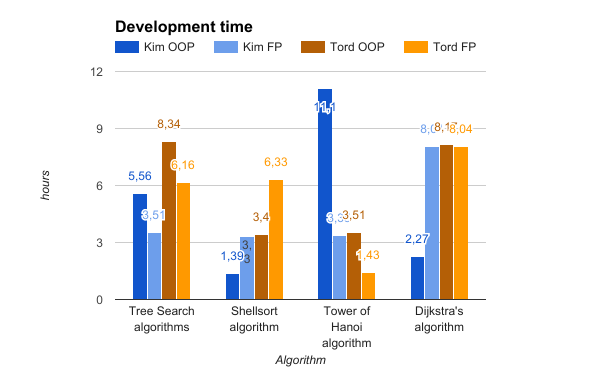
\includegraphics[width=\textwidth]{development-time-graph}

\caption{Development time for our implementations}
\label{fig:development-time-graph}
\end{figure}
\subsection{Lines of code}
The total results for the lines of code were:
\begin{description}
\item[Kim OOP] - 930 lines of code.
\item[Kim FP] - 618 lines of code.
\item[Tord OOP] - 703 lines of code.
\item[Tord FP] - 530 lines of code.
\end{description}

For both Kim and Tord the functional implementations had less code in total and individually for all implementations except for the Shellsort algorithm, see figure~\ref{fig:lines-of-code-graph}. For the Shellsort algorithm both OOP implementations had the least code. 

We can see for Kim's Tower of Hanoi algorithm that there is a large difference in code length between the OOP and the FP implementations. This is because of her choice to using classes to represent the Tower of Hanoi game, pegs and discs rather than just using arrays.

We expected that the functional implementations would produce less code than the object-oriented implementations. The functional implementations did, for all algorithms except for Shellsort, have less code because we did not implement classes. This gave us less code, but we both think that this does not increase readability. Classes add a layer of abstraction that we both found useful for writing our own code and understanding each other's.

\begin{figure}[H]
\centering
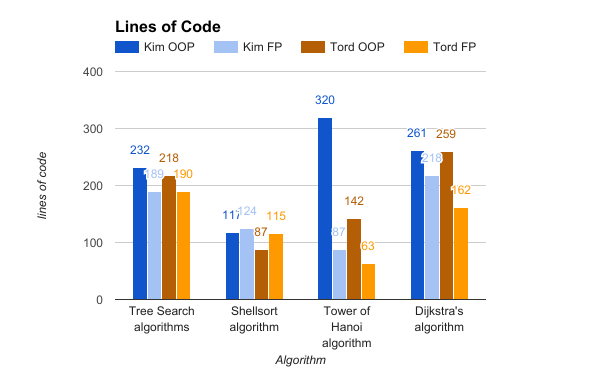
\includegraphics[width=\textwidth]{lines-of-code-graph}

\caption{Lines of code in our implementations}
\label{fig:lines-of-code-graph}
\end{figure}
\subsection{Binary Search Tree Algorithms}
In figure~\ref{fig:binary-tree-runtime} and figure~\ref{fig:binary-tree-memory} we can see that for Kim the functional implementation has a better execution time, but still uses a lot more memory than the object-oriented implementation. Tord's object-oriented implementation performs a lot better than his functional, both for memory usage and execution time. Tord's functional implementation is a lot slower and uses a lot more memory than all the other implementations.

Kim's functional implementation is faster than her object-oriented, since her inOrderTraversal-function is unnecessarily complex and does not fully utilize the idea of the recursive algorithm seen in section~\ref{sec:binary-tree}. Her recursive algorithm uses more memory because we are handling our data structures as immutable. This means that we are copying our data structures recursively when initiating an array or a tree, which JavaScript handles by placing all these copies into memory. We suspect that this would have looked different in other languages that support immutable data structures. 

The reason that Tord’s functional algorithm is so much slower is that he used arrays instead of native objects. The problem with arrays is not the array itself but how it is used for the algorithm. The child nodes are placed in the array at \(n * 2 + 1\) or \(n * 2 + 2\), where n is the parent's index. This made the array much bigger than necessary. 

Overall our results suggest that it is possible to write good algorithms in both paradigms, but OOP has the upper hand since it is using significantly less memory than FP.

\begin{figure}[H]
\centering
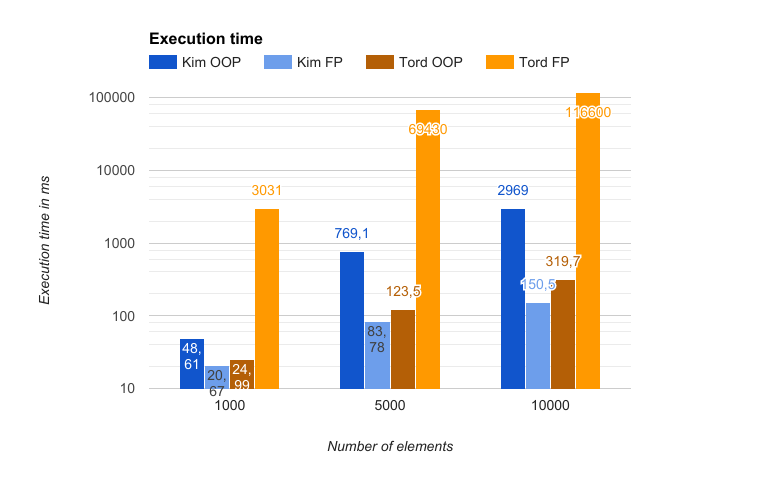
\includegraphics[width=\textwidth]{binary-tree-runtime}

\caption{Execution time for binary search tree implementations.}
\label{fig:binary-tree-runtime}
\end{figure}

\begin{figure}[H]
\centering
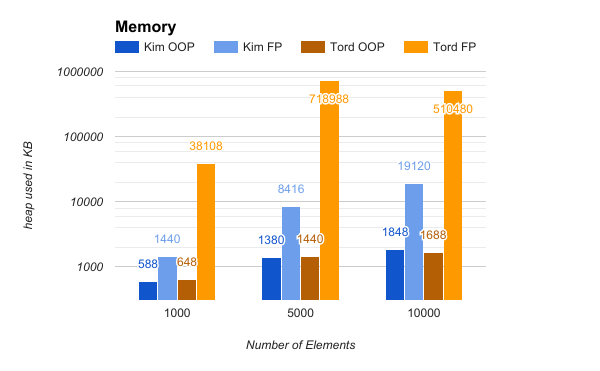
\includegraphics[width=\textwidth]{binary-tree-memory}

\caption{Memory usage for binary search tree implementations.}
\label{fig:binary-tree-memory}
\end{figure}
\subsection{Shellsort}
\label{sec:shellsort-results}
For Shellsort Kim's and Tord's results are following the same trend, see figure~\ref{fig:shellsort-runtime} and figure~\ref{fig:shellsort-memory}. Both of their OOP implementations performed a lot better with faster execution times and lower memory usage. As seen in figure~\ref{fig:development-time-graph} and figure~\ref{fig:lines-of-code-graph} both OOP implementations also had less code and a shorter development time than the FP implementations.

The reason that the functional and object-oriented implementations were very similar in code length is that there were not many classes to implement in the object-oriented solution. Working with and copying arrays recursively is also a lot slower, probably because of the high memory usage and JavaScript's garbage collection that has to keep collecting when the memory usage is too high.

\begin{figure}[H]
\centering
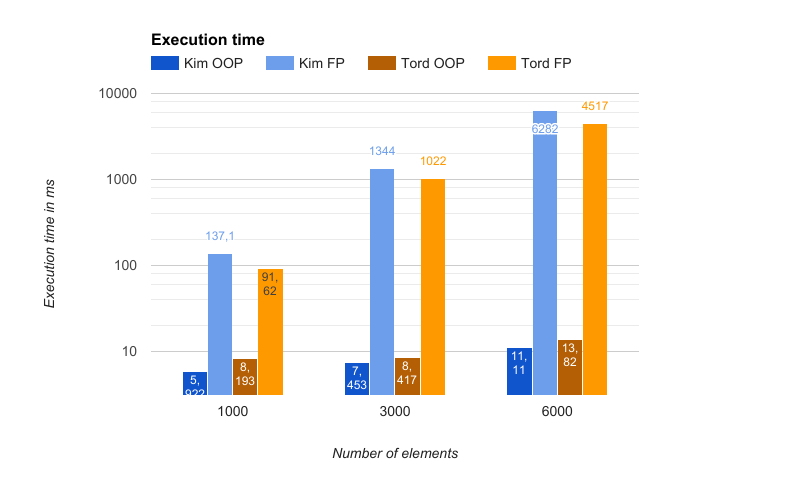
\includegraphics[width=\textwidth]{shellsort-runtime}

\caption{Execution time for the Shellsort implementations.}
\label{fig:shellsort-runtime}
\end{figure}

\begin{figure}[H]
\centering
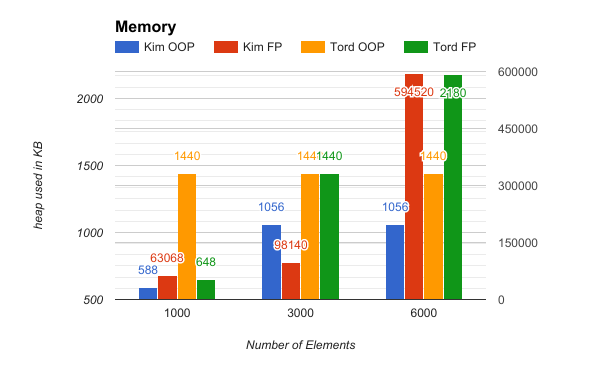
\includegraphics[width=\textwidth]{shellsort-memory}

\caption{Memory usage for the Shellsort implementations.}
\label{fig:shellsort-memory}
\end{figure}
\subsection{Tower of Hanoi}
In figure~\ref{fig:hanoi-runtime} and figure~\ref{fig:hanoi-memory} we can see that Kim's functional implementation was both faster and used less memory than her object-oriented implementation. However, there was not as big of a difference in performance between the two compared to results for other implementations. Tord's object-oriented implementation was a lot faster and used a lot less memory than all the others, while his functional implementation was the slowest and used the most memory.

Tord had to change the object-oriented implementation of this algorithm after we had analysed the results. This was because during the first measurement runs this implementation ran out of memory with 25 elements and was significantly slower than it is currently. This resulted in that his implementation was improved after we analyzed the first results, which might have decreased the time he had to spend. On the other hand it shows us that it is easy for small mistakes to have a large impact on performance when handling larger data sizes. This was also the algorithm where Tord searched for help online, which might also have resulted in that it is more effective than the other implementations.
 
\begin{figure}[H]
\centering
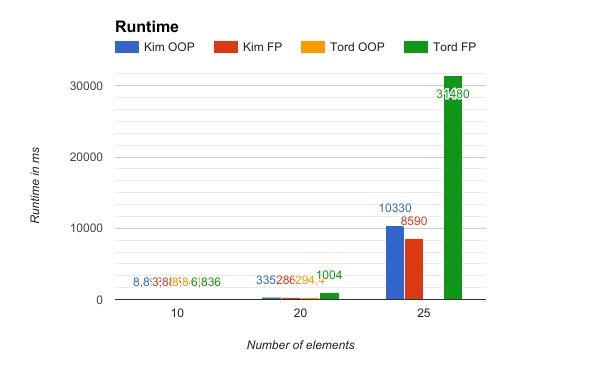
\includegraphics[width=\textwidth]{hanoi-runtime}

\caption{Execution time for the Tower of Hanoi implementations.}
\label{fig:hanoi-runtime}
\end{figure}

\begin{figure}[H]
\centering
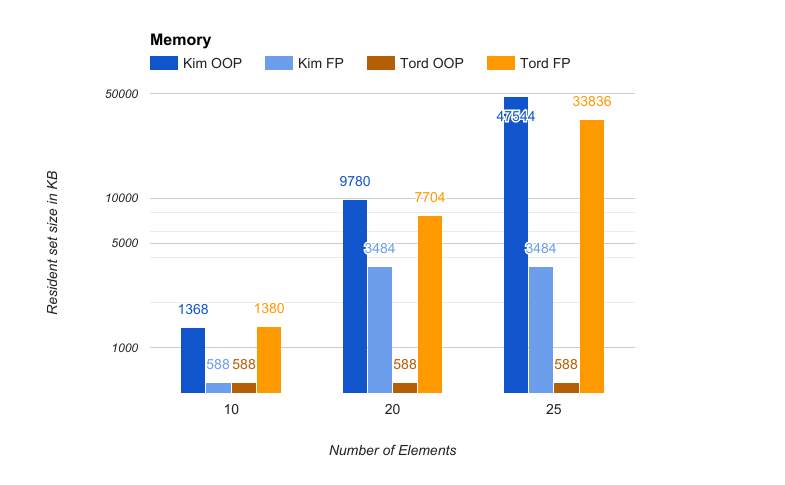
\includegraphics[width=\textwidth]{hanoi-memory}

\caption{Memory usage for the Tower of Hanoi implementations.}
\label{fig:hanoi-memory}
\end{figure}
\subsection{Dijkstra's algorithm}
Both Kim's and Tord's object-oriented implementations performed better than their functional implementations for Dijkstra's algorithm. Kim's functional implementation was a lot slower than all the others, while Tord's functional implementation only performed slightly worse than his object-oriented implementation, see figure~\ref{fig:dijkstras-runtime} and figure~\ref{fig:dijkstras-memory}. 

As expected the object-oriented implementations performed better for this algorithm. However, Kim's functional implementation is a lot slower and uses a lot more memory than the others. This is because she chose to represent edges as an object where the keys were the edges and the values were the weight. For example:

\begin{lstlisting}[language=Pascal]
var edges = {
	'node1-node2': 9
	'node2-node3': 3
}
\end{lstlisting}

She used JavaScript's Object.keys() function, see \cite{jsref}, to get an array with the keys and then processed that to get the wanted edges. This adds a lot of copying and handling of objects and arrays, which in turn results in a higher memory usage and more garbage collecting, which leads to a slower execution time.

\begin{figure}[H]
\centering
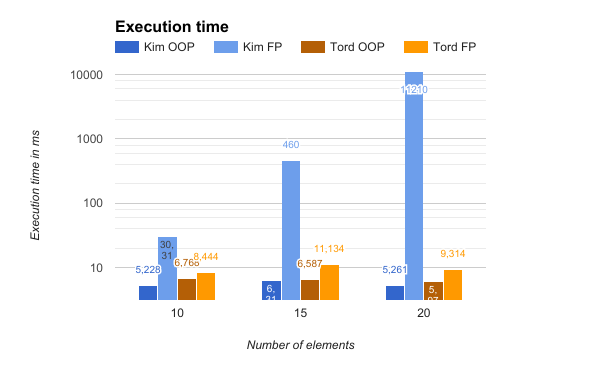
\includegraphics[width=\textwidth]{dijkstras-runtime}

\caption{Execution time usage for Dijkstra's algorithm implementations.}
\label{fig:dijkstras-runtime}
\end{figure}

\begin{figure}[H]
\centering
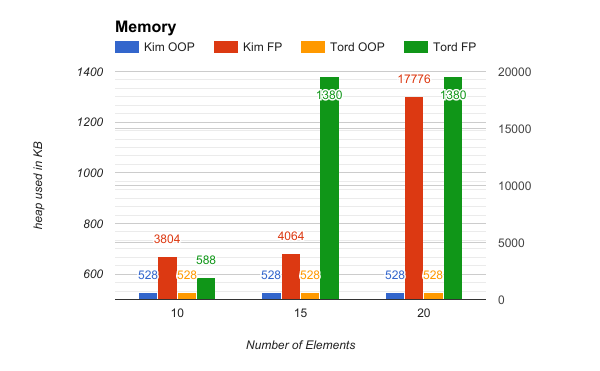
\includegraphics[width=\textwidth]{dijkstras-memory}

\caption{Memory usage for Dijkstra's algorithm implementations.}
\label{fig:dijkstras-memory}
\end{figure}

\section{Discussion}
Most of the implementations are faster when implemented in their expected way. For example, the binary search tree algorithms have a faster execution time when implemented recursively and the Shellsort algorithm has faster execution time when implemented iteratively. The development time results also follow this pattern. We spent more time when implementing, for example, Shellsort recursively or the Tower of Hanoi iteratively. 

We expected the development time to be shorter for the object-oriented implementations, since we both have had prior experience with it and since we have nearly no prior experience with functional programming. The results show that this was not necessarily so. Neither of the paradigms seem significantly faster to implement, however the functional paradigm might have a slight upper hand since we both had no prior experience with it. 

For the execution time results, we did expect the object-oriented implementations to be faster than the functional implementations, based on this study comparing functional and object-oriented languages \cite{hasmadole} and our research about JavaScript, see section~\ref{sec:javascript}. Overall the functional implementations performed worse than the object-oriented implementations. We both implemented very slow implementations when using functional approaches, compared to when we implemented slow implementations according to OOP.

Since we only had two different test groups with one person in each, it was difficult to analyze our results when algorithms were hard to compare. For example when an algorithm was much slower than all the others. This might not be because of the paradigm itself, but rather because the programmer has made a mistake. However, it can still give us some results as to if it is easier to make mistakes in one paradigm, but that would only be valid for that particular language. We think that it would be possible to draw more conclusions if there were more test subjects taking part in this experiment.

Our results suggest that the paradigm methods themselves, such as using classes with methods or avoiding side effects, do not necessarily have a large impact on the performance. In some cases, for example our Shellsort implementation results in section~\ref{sec:shellsort-results}, FP clearly performs worse than OOP. Shellsort requires a lot of hiding state and handling data structures as immutable, which is slow and memory consuming in JavaScript. Optimizing functional solutions is an option, but that would take additional time and would have to be considered when developing functional JavaScript. Perhaps using one of the functional libraries available solves this problem.

Overall we both appreciated trying out functional programming, but we don't think that we will use pure functional programming or functional languages in the future if we don't have to. We will, however, use a lot of the approaches that we have been using in this experiment. In our experience we found that we had less bugs when avoiding side effects and the functions were modular and easy to combine. We also liked using classes since there was a layer of abstraction on top of JavaScript's native types. We think that combining the two paradigms and using recursion or iteration when it fits best would benefit both the performance, development time and code readability. 
\section{Conclusion}
As we expected, our object-oriented implementations performed better than our functional implementations, while our functional implementations had a shorter development time and less code. This was the case, even though we did not have any earlier experience with functional programming.  

Based on our results, different paradigms are good for different things and one is not clearly better than the other. According to our research most languages perform well, and there are also a lot of multiparadigm languages out there. Our conclusion is that it is best to use a combination of the paradigms if possible. Especially since functional programming and object-oriented programming are not opposites. We think that object-oriented programmers would benefit from using methods from FP, even if they work in a more object-oriented language. To us it makes sense that a lot of the object-oriented languages, that are based on the imperative paradigm, are starting to implement support for functional approaches.

\section{Future Work}
In this experiment we have implemented the algorithms ourselves and compared our own work. It would be interesting to see a similar experiment with multiple test subjects that are not involved in the thesis work. 

A lot of our sources argue that functional programming should be really good for handling data concurrently. Therefore an experiment to compare different paradigms,  when implementing concurrent and asynchronous algorithms, from both a performance, development and maintainability perspective would be interesting. 

We also did these implementations in JavaScript. It would be interesting to see this kind of comparison in another language that better support full functional or full OOP approaches. Perhaps comparing other paradigms and a combination of paradigms as well.

\bibliographystyle{IEEEtran}
\bibliography{IEEEabrv,references}
\appendix
\section{Appendix}
\label{appendix:test-cases}
In the following appendices, you will find our test cases and images describing the test data.
\subsection{Test cases}
All the images referenced in this appendix can be found in appendix~\ref{test-case-images}
\begin{table}[H]
\caption{Binary search tree algorithms insert tests}
\begin{tabular}{ | l p{10cm} | }
\hline
ID & T1 \\
Algorithm & Binary search tree algorithms \\
Function & insert(comparable, rootNode) \\
Description & Inserted items should be added at the correct place in the tree. If number already exists in the binary search tree, it should not be inserted. \\
Preconditions & See figure~\ref{fig:input-tree} \\
\hline
ID & T1.1 \\
Input & 9, node(13) \\
Expected values & FP: None, OOP: See figure~\ref{fig:input-tree} \\
Expected output & FP: See figure~\ref{fig:input-tree}, OOP: false \\
\hline
ID & T1.2 \\
Input & 8, node(13) \\
Expected values & FP: None, OOP: See figure~\ref{fig:output-tree-8} \\
Expected output & FP: See figure~\ref{fig:output-tree-8}, OOP: true \\
\hline
ID & T1.3 \\
Input & 1, node(13) \\
Expected values & FP: None, OOP: See figure~\ref{fig:output-tree-1} \\
Expected output & FP: See figure~\ref{fig:output-tree-1}, OOP: true \\
\hline
ID & T1.2 \\
Input & 33, node(13) \\
Expected values & FP: None, OOP: See figure~\ref{fig:output-tree-33} \\
Expected output & FP: See figure~\ref{fig:output-tree-33}, OOP: true \\
\hline
\end{tabular}
\label{tab:insert-tests}
\end{table}

\begin{table}[H]
\caption{Binary search tree algorithms findNode tests}
\begin{tabular}{ | l p{10cm} | }
\hline
ID & T2 \\
Algorithm & Binary search tree algorithms \\
Function & findNode(comparable, rootNode) \\
Description & findNode should return the node containing comparable. If comparable is not in the tree undefined should be returned. \\
Preconditions & See figure~\ref{fig:input-tree} \\
\hline
ID & T2.1 \\
Input & 5, node(13) \\
Expected values & None \\
Expected output & undefined \\
\hline
ID & T2.2 \\
Input & 13, node(13) \\
Expected values & None \\
Expected output & node(13) \\
\hline
ID & T2.3 \\
Input & 2, node(13) \\
Expected values & None \\
Expected output & node(2) \\
\hline
ID & T2.4 \\
Input & 32, node(13) \\
Expected values & None \\
Expected output & node(32) \\
\hline
ID & T2.5 \\
Input & 20, node(13) \\
Expected values & None \\
Expected output & node(20) \\
\hline
\end{tabular}
\label{tab:find-node-tests}
\end{table}

\begin{table}[H]
\caption{Binary search tree algorithms inOrderTraversal tests}
\begin{tabular}{ | l p{10cm} | }
\hline
ID & T3 \\
Algorithm & Binary search tree algorithms \\
Function & inOrderTraversal() \\
Description & Should return a sorted array of the elements in the tree. If the tree is it should return an empty array. \\
\hline
ID & T3.1 \\
Preconditions & See figure~\ref{fig:input-tree} \\
Input & FP: node(13), OOP: none \\
Expected values & None \\
Expected output &  [2, 3, 6, 7, 9, 13, 16, 20, 24, 32] \\
\hline
ID & T3.2 \\
Preconditions & Empty tree \\
Input & FP: none, OOP: none \\
Expected values & None \\
Expected output & [] \\
\hline
\end{tabular}
\label{tab:traversal-tests}
\end{table}

\begin{table}[H]
\caption{Shellsort algorithm tests}
\begin{tabular}{ | l p{10cm} | }
\hline
ID & T4 \\
Algorithm & Shellsort \\
Function & Shellsort(array) \\
Description & If an array of numbers is input a sorted array should be returned. If an empty array is input an empty array should be returned. \\
Preconditions & None \\
\hline
ID & T4.1 \\
Input & [] \\
Expected values & None \\
Expected output &  [] \\
\hline
ID & T4.2 \\
Input & [ 9, 8, 1, 15, 3, 4, 11, 2, 7, 6] \\
Expected values & None \\
Expected output & [ 9, 8, 1, 15, 3, 4, 11, 2, 7, 6] \\
\hline
\end{tabular}
\label{tab:shellsort-tests}
\end{table}

\begin{table}[H]
\caption{Tower of Hanoi algorithm tests}
\begin{tabular}{ | l p{10cm} | }
\hline
ID & T5 \\
Algorithm & The Tower of Hanoi \\
Function &  hanoi(tower, start, dest, aux) \\
Description & Should return start, dest and aux pegs with moved tower. If tower has zero discs it should return empty start, dest and aux. The algorithm should take \(2^n - 1\) moves.\\
Preconditions & None \\
\hline
ID & T5.1 \\
Input & tower size 8, peg1 with tower, peg3 empty, peg2 empty \\
Expected values & FP: none, OOP: nrOfMoves=255 \\
Expected output &  peg1 empty, peg2 empty, peg3 with tower \\
\hline
ID & T5.2 \\
Input & tower size 0, peg1 empty, peg3 empty, peg2 empty \\
Expected values & FP: none, OOP: nrOfMoves=0 \\
Expected output & peg1 empty, peg2 empty, peg3 empty \\
\hline
\end{tabular}
\label{tab:tower-of-hanoi-tests}
\end{table}

\begin{table}[H]
\caption{Dijkstra's algorithm tests}
\begin{tabular}{ | l p{10cm} | }
\hline
ID & T6 \\
Algorithm & Dijksta's algorithm \\
Function & dijkstras(graph, startNode, endNode) \\
Description & Should return the shortest path from startNode to endNode. If startNode is same as endNode it should return empty path. If graph is empty it should return empy path.\\
Preconditions & None \\
\hline
ID & T6.1 \\
Input & See figure~\ref{fig:input-graph}, node1, node6 \\
Expected values & None \\
Expected output &  See figure~\ref{fig:output-graph} \\
\hline
ID & T6.2 \\
Input & See figure~\ref{fig:input-graph}, node1, node4 \\
Expected values & None \\
Expected output &  See figure~\ref{fig:output-graph2} \\
\hline
ID & T6.3 \\
Input & See figure~\ref{fig:input-graph}, node2, node5 \\
Expected values & None \\
Expected output &  See figure~\ref{fig:output-graph3} \\
\hline
ID & T6.4 \\
Input & See figure~\ref{fig:input-graph}, node1, node1\\
Expected values & None \\
Expected output & empty path \\
\hline
ID & T6.5 \\
Input & nodes=[], edges[], noNode, noNode \\
Expected values & None \\
Expected output & empty path \\
\hline
\end{tabular}
\label{tab:dijkstras-tests}
\end{table}
\subsection{Test case images}
\label{test-case-images}
\begin{figure}[H]
\centering
\includegraphics[width=0.9\textwidth]{input-tree}

\caption{Input tree}
\label{fig:input-tree}
\end{figure}

\begin{figure}[H]
\centering
\includegraphics[width=0.9\textwidth]{output-tree-8}

\caption{Output tree after inserting 8}
\label{fig:output-tree-8}
\end{figure}

\begin{figure}[H]
\includegraphics[width=\textwidth]{output-tree-1}

\caption{Output tree after inserting 1}
\label{fig:output-tree-1}
\end{figure}

\begin{figure}[H]
\includegraphics[width=\textwidth]{output-tree-33}

\caption{Output tree after inserting 33}
\label{fig:output-tree-33}
\end{figure}

\begin{figure}[H]
\centering
\includegraphics[width=0.9\textwidth]{input-graph}

\caption{Input graph}
\label{fig:input-graph}
\end{figure}

\begin{figure}[H]
\centering
\includegraphics[width=0.8\textwidth]{output-graph}

\caption{Output graph 1}
\label{fig:output-graph}
\end{figure}

\begin{figure}[H]
\centering
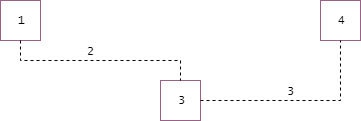
\includegraphics[width=0.6\textwidth]{output-graph2}

\caption{Output graph 2}
\label{fig:output-graph2}
\end{figure}

\begin{figure}[H]
\centering
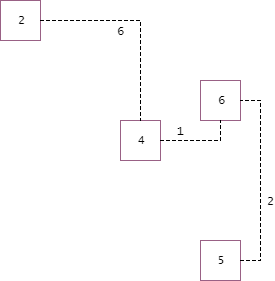
\includegraphics[width=0.5\textwidth]{output-graph3}

\caption{Output graph 3}
\label{fig:output-graph3}
\end{figure}

\end{document}

